\documentclass[12pt, a4paper]{article}
\usepackage[utf8]{inputenc}
\usepackage[margin=1.2in]{geometry}
\usepackage{listings}
\usepackage{setspace}
\usepackage{xcolor}
\usepackage{titlesec}
\usepackage{enumitem}
\usepackage{amssymb}
\usepackage{amsmath}
\usepackage{tocloft}
\usepackage{bm}
\usepackage{multicol}
\usepackage{graphicx}
\graphicspath{{./Figures/}}
\usepackage{color}
\usepackage{hyperref}
\hypersetup{
	colorlinks=true,
	linkcolor=blue,
	urlcolor=blue,
	linktoc=none
}
\titleformat*{\section}{\Large\bfseries}
\titleformat*{\subsection}{\large\bfseries}
\renewcommand\thesection{\Roman{section}.}
\renewcommand\thesubsection{\alph{subsection}.}
\addtolength{\cftsecnumwidth}{16pt}

\begin{document}
\begin{spacing}{1.1}

	\begin{titlepage}
		\begin{center}
			\vspace*{1.4cm}
			
			\Huge \textbf{Capstone Project Report}
			
			\vspace*{1cm}
			
			
\includegraphics[scale=.5]{logo}
			
			\vspace*{1cm}
			
			\LARGE {Udacity Machine Learning Engineer Nanodegree}
			
			\vspace*{1cm}
			
			\hrule \vspace*{.5cm}
			
			\Large \textbf{A capstone report for analyzing worldwide food production and population from 1961-2013.}
			
			\vspace*{.5cm} \hrule
			
			\vspace*{1cm}
			
			\Large Derek Helms \\
			\Large January 25$^{th}$, 2021
		\end{center}
	\end{titlepage} \newpage

	\begin{titlepage}
		\vspace*{3cm}
		\renewcommand*\contentsname{Table of Contents}
		\tableofcontents
	\end{titlepage} \newpage

%%%% PAGE 1 %%%%

	\section{Definition}
	\subsection{Project Overview}
	The current world population is nearly 7.8 billion people, and this number is estimated to rise to around 9.7 billion in the year 2050. This means within the next 30 years, we will need to feed two billion more people without sacrificing the planet (1). This means we will need to double our crop production in order to feed that growing population. Agriculture is one of the greatest contributors of global warming, with farming consuming immense amounts of our water supplies and leaving major pollutants as its byproduct from fertilizer runoff (4). \vspace*{2mm}\\	
	Two different datasets were used in the analysis, one coming from \href{https://www.kaggle.com/dorbicycle/world-foodfeed-production}{Kaggle} and one coming from \href{http://www.fao.org/faostat/en/#data/OA}{FAO} (the Food and Agriculture Organization of the United Nations).\vspace*{2mm}\\	
	The dataset obtained through Kaggle is a Food Balance Sheet that originated from FAO's database, but has been formatted for easy of use, with a total of 63 features and 21477 observations. Food Balance Sheets represent the pattern of a country's food supply during a period of time, in this case it is yearly from 1961 to 2013, and measured in 1000 tonnes (2)
	\begin{center}	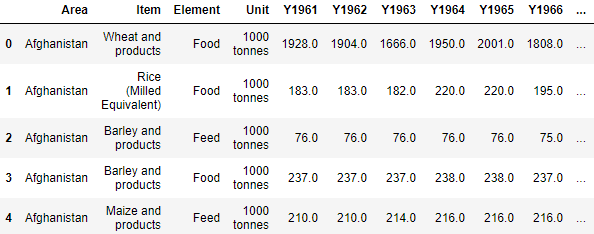
\includegraphics[scale=.9]{food_data}	\end{center}
	The dataset obtained through FAO is a time series dataset that contains the estimated/projected population (for both sexes) in each country from 1961 to 2018. The estimates are based on data from the World Population Prospects and World Urbanization Prospects (3).
	\begin{center}	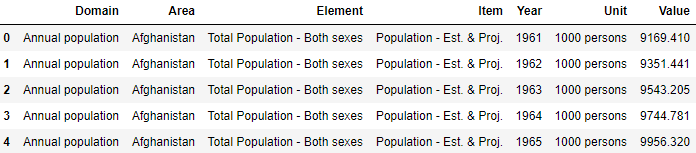
\includegraphics[scale=.8]{pop_data}	\end{center} \newpage

%%%% PAGE 2 %%%%

	\noindent The use cases for each dataset is as follows. The Kaggle dataset will be used in analyzing food production, seeing which countries produce the most and if it is for human or livestock consumption. This data will also be used to cluster countries together based on their production levels, ideally separating high and low producing countries. The FAO dataset will be used to compare the global population to the yearly total food production, as well as further analyzing the highest producing countries to see if they have the largest/fastest increasing populations.	
	
	\subsection{Problem Statement}
	With a continuously growing population this leads to the question, how do we supply the necessary amount of food for an increasing world population without sacrificing the climate of our planet? There are many solutions to this question, but the focus of this capstone will be on analyzing the global production of consumables, as well as the ratio of food (human consumption) to feed (livestock consumption) produced by each country. Only 55\% of the current world crop production is consumed by humans, with the remaining being fed to livestock. On top of this, nearly 25\% of the world's food calories are wasted before they can be consumed (4).\vspace*{2mm}\\	
	One aspect to explore is which food items are the most produced and the use case for those food items, whether they are for human or animal consumption. This will allow us to understand where a majority of our food is being directed, and as suggested by \href{https://www.nationalgeographic.com/foodfeatures/feeding-9-billion/}{National Geographic}, could a shift in diet lead to more crops being used for human consumption rather than livestock feed. Creating graphs to find insight will allow us to see how population change has correlated to food production, and what percentage of consumables are for humans compared to livestock. \vspace*{2mm}\\	
	The second aspect to explore is creating a linear model that can estimate the total global production needed for a given global population. This means correlating population and production in order to create a regression model that can predict the necessary production for the 2050 population. These will be compared to scientific articles that determine the necessary growth in production needed, and which model best fits these predictions.\vspace*{2mm}\\
	The last aspect of the data to explore is separating the countries into clusters based on their yearly production. Analyzing which countries are responsible for feeding the majority of the population, and how to ensure they can continue to do so. From this, we can also see which countries are not highly producing, and how we can aid them in increasing production if possible. \newpage

%%%% PAGE 3 %%%%

	\subsection{Metrics}
	To evaluate our graphing and data exploration, we can use the \href{http://www.fao.org/faostat/en/#rankings/countries_by_commodity}{FAO rankings} for countries by commodity, which we can then compare to our graphs to see if we have the data correctly labeled. This ranking allows us to see the top 20 country's that produce the most for each food item, as well as the top 20 food items produced by each country from the years 1961 to 2019.\vspace*{2mm}\\
	To evaluate our regression, we will use the root mean squared error (RMSE), in order to determine which line is best fitting our data. However, the 2050 estimate will also be used in determining the evaluation of the model in order to avoid overfitting the original data and having a poor future estimate (since we know the production needs to be anywhere for 50-100\% increased). \vspace*{2mm}\\
	With the data being unlabeled, it will be difficult to ensure that our clusters are properly partitioned. However, we can analyze both the clusters and graphs we create using two separate methods. One metric we can use to evaluate our model will be a \href{https://scikit-learn.org/stable/auto_examples/cluster/plot_kmeans_silhouette_analysis.html}{silhouette score}, which will measure on a scale from [-1,1] how close each point on one cluster is to points in the neighboring clusters. We will want to aim for a silhouette coefficient near +1 to indicate that our samples are far away from neighboring clusters (5). \vspace*{2mm}\\
	To evaluate our graphing and data exploration, we can use the \href{http://www.fao.org/faostat/en/#rankings/countries_by_commodity}{FAO rankings} for countries by commodity, which we can then compare to our graphs to see if we have the data correctly labeled. This ranking allows us to see the top 20 country's that produce the most for each food item, as well as the top 20 food items produced by each country from the years 1961 to 2019. \vspace*{2mm}
	
	\section{Analysis}
	This is where the majority of the project has taken place, in exploring the data and creating visualizations in order to determine where the food we are producing is going, as well as who is responsible for producing it. The analysis was broken down into two different sections: production and population exploration. In the production section, we analyzed the top producing countries, explored the top produced food items, and finally the use case for the food items (food vs feed). In the population section, we analyzed population vs production, the populations for the top producing countries, and the largest population changes over the last 53 years. A more in-depth description and visualization will be given in the following two subsections. \newpage

%%%% PAGE 4 %%%%
	
	\subsection{Production Exploration}
	\textbf{Top 10 Producing Countries:}\\
	To begin the exploration, we wanted to graph the top 10 producing countries for global production from 1961 to 2013. After this, we compared total production for a given number of top countries to the rest of the world to see how much global production each are responsible for.
	\begin{center}
	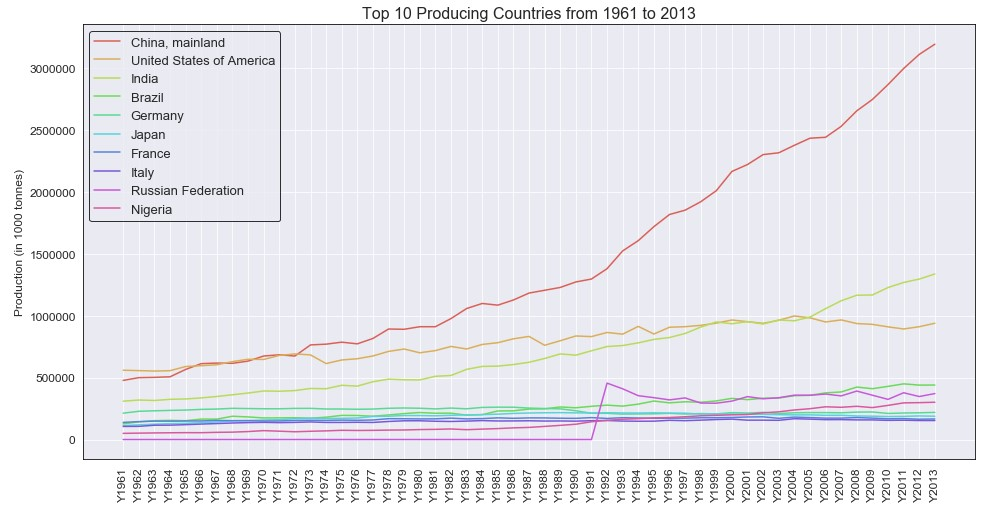
\includegraphics[scale=.58]{top_20_c_yearly} \vspace*{2mm}\\
	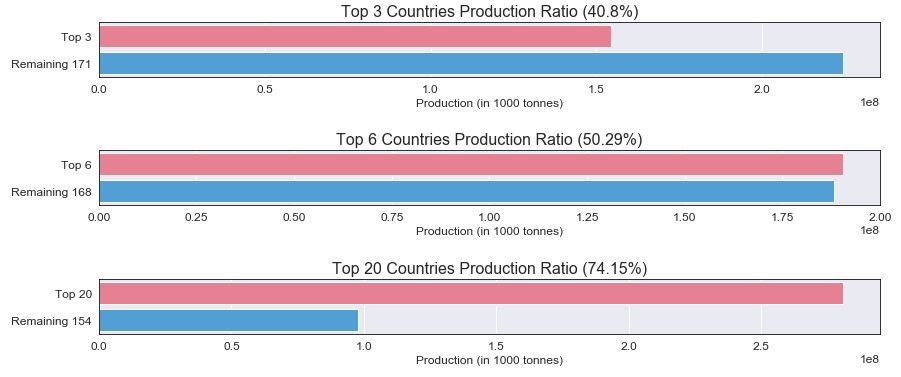
\includegraphics[scale=.58]{top_20_c_total}
	\end{center}
	From the line graph, we can see that the top 3 countries have been the top producers over the last 53 years. With China becoming dominant in the year 1972, it looks to be the beginning of an exponential growth pattern. The United States was second to China for a majority of the data, but seems to have plateaued and been passed by India starting in the early 2000's. India, being third highest of the data, has begun growing quickly since the late 1980's and seems to be increasing similar to China. An interesting finding is the Russian Federation spiking from 0 to nearly 500,000,000 tonnes of production from 1991 to 1992. \newpage

%%%% PAGE 5 %%%%
	
	\noindent This was due to the fact that the Russian Federation was found on December 25, 1991 and this was when our data begun with them (no production for Soviet Union was recorded in our data, which was the old name).\vspace*{2mm}\\
	Looking at the bar charts, and adding the three top producing countries together, it seems that they are responsible for around 40\% of the total global production. Going further, we can see that the top 6 producing countries are responsible for over 50\% of the global production, and the top 20 being responsible for 74\%. Out of 174 countries, it seems that only a small amount of them are responsible for the vast majority of production (however, these countries populations are also much larger than the others). \vspace*{6mm}\\
	\textbf{Exploring China's Production:}\\
	Being the top producer over the last 53 years (and most likely much before then), we want to further look into the production of the ``China, mainland" area. We will want to see what products make up a majority of their production, as well as the yearly breakdown to see any trends in production.
	\begin{center}
	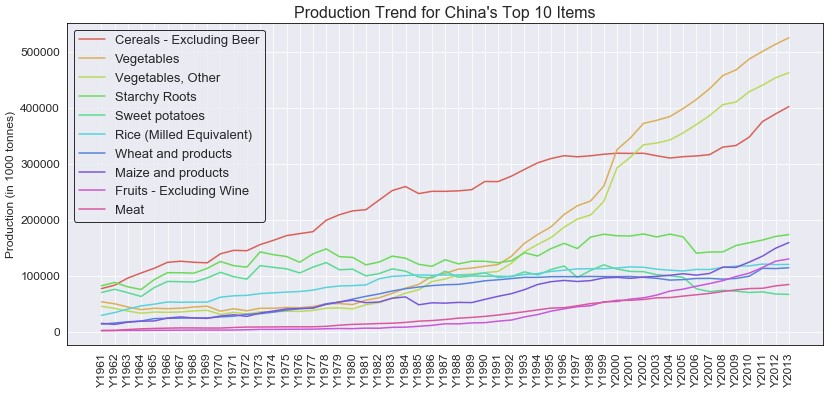
\includegraphics[scale=.65]{china_prod} 
	\end{center}
	From the graphs, we see that historically \textit{Cereals - Excluding Beer} has been the dominant product for China, but recently there has been a large spike in \textit{Vegetables} and \textit{Vegetables, Other} that has surpassed Cereals starting in the year 2000. However, Cereals seem to be rising again and could become the most produced item if Vegetables plateau. This is important to keep in min for the next section of the exploration, where we looked at the top produced foot items. \newpage
	
%%%% PAGE 6 %%%%

	\noindent \textbf{Top Produced Items:}\\

	
	
	\newpage
	
%%%% PAGE 4 %%%%
	
	
	
	
	
	
	
	
	
	\newpage
	
%%%% RESOURCES %%%%

	\section{Resources}
	$[1]$ Oppenheim, Dor. ``Who Eats the Food We Grow?" \textit{Kaggle}, 30 Nov. 2017, \\ \hspace*{5mm} www.kaggle.com/dorbicycle/world-foodfeed-production. \vspace*{2.5mm}\\
	$[2]$ ``Food Balances (Old Methodology and Population)." \textit{FAOSTAT}, Food and \\ \hspace*{5mm} Agriculture Organization of the United Nations, 12 Dec. 2017, \\ \hspace*{5mm} www.fao.org/faostat/en/\#data/FBSH. \vspace*{2.5mm}\\
	$[3]$ ``Annual Population." \textit{FAOSTAT}, Food and Agriculture Organization of the \\ \hspace*{5mm} United Nations, 16 Dec. 2019, www.fao.org/faostat/en/\#data/OA. \vspace*{2.5mm}\\
	$[4]$ Foley, Jonathan. ``A Five-Step Plan to Feed the World." \textit{Feeding 9 Billion - \\ \hspace*{5mm} National Geographic}, www.nationalgeographic.com/foodfeatures/feeding-9-billion/.\vspace*{2.5mm}\\
	$[5]$ ``Selecting the Number of Clusters with Silhouette Analysis on KMeans \\ \hspace*{5mm} Clustering." \textit{Scikit}, 
	\\ \hspace*{6mm} scikit-learn.org/stable/auto\_examples/cluster/plot\_kmeans\_silhouette\_analysis.html.\vspace*{2.5mm}\\
	$[6]$ Kiersz, Andy. ``The World Could Have Another Billion People in Thirteen \\\hspace*{6mm}Years." \textit{Business Insider}, Business Insider, 29 July 2015,\\\hspace*{6mm}www.businessinsider.com/un-world-population-projections-2015-7. \vspace*{2.5mm}\\
	


\end{spacing}
\end{document}